\begin{minipage}[c]{0.47\linewidth}
\centering
\small
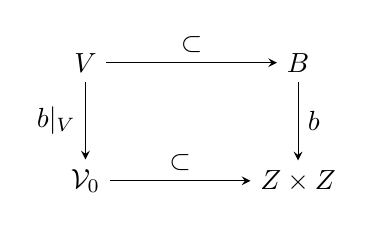
\begin{tikzpicture}[>=stealth, baseline=(current bounding box.center)]
\node (v) at (0,1.5) {$V$};
\node (b) at (2.7,1.5) {$B$};
\node (v0) at (0,0) {$\mathcal V_0$};
\node (zz) at (2.7,0) {$Z\times Z$};
\draw[->] (v)--node[above] {$\subset$} (b);
\draw[->] (v0)--node[above] {$\subset$} (zz);
\draw[->] (v)--node[left] {$b|_V$} (v0);
\draw[->] (b)--node[right] {$b$} (zz);
\end{tikzpicture}
\[
 \begin{gathered}
 V_z=\operatorname{Bl}_xX,\\
 (V\cap E)_z=\mathbb P(T_z^*D_\lambda)
       \subset E_z=\mathbb P(T_z^*Z).
 \end{gathered}
\]
\end{minipage}
\hfill
\begin{minipage}[c]{0.50\linewidth}
\centering
\small
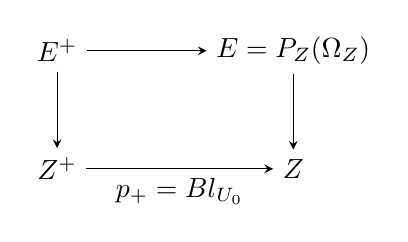
\begin{tikzpicture}[>=stealth, baseline=(current bounding box.center)]
\node (ep) at (0,1.5) {$E^+$};
\node (e) at (3,1.5) {$E=\mathbb P_Z(\Omega_Z)$};
\node (zp) at (0,0) {$Z^+$};
\node (z) at (3,0) {$Z$};
\draw[->] (ep)--(e);
\draw[->] (ep)--(zp);
\draw[->] (e)--(z);
\draw[->] (zp)--node[below] {$p_+=\operatorname{Bl}_{U_0}$} (z);
\end{tikzpicture}
\[
 \begin{gathered}
 J_+=p_+^{-1}(U_0),\qquad U_0=X\times\mathbb P^1,\\
 \mathcal J=(\mathcal I_V\cdot\cO_E)\cdot\cO_{E^+}.
 \end{gathered}
\]
\end{minipage}
